\chapteropen{Chapter 4: Conceptual models and class diagrams}{chapter-4}
\markboth{Ch. 4 | Class diagrams}{}


\begin{studycolumns}
\vspace{0pt}
\begin{eli5box}
Think of a cinema: a TicketScreen talks to the customer, a BookingController organises the booking and a Ticket stores a booking fact. A class is a kind of thing; an object is one particular instance. A link's numbers tell you how many objects can be connected, not which class owns the drawing.
\end{eli5box}
\textbf{Answer check:} Separate boundaries, coordinating controls and persistent entities. Conceptual questions may prohibit attributes/operations; add them only for detailed design. State invariants that multiplicities cannot express, such as one active hold despite many historical holds.
\end{studycolumns}

\subsection*{Visual: assign each class a responsibility}
\sectionlabel{h-visual-assign-each-class-a-responsibility}


\par\smallskip\noindent\begin{minipage}{\linewidth}\centering
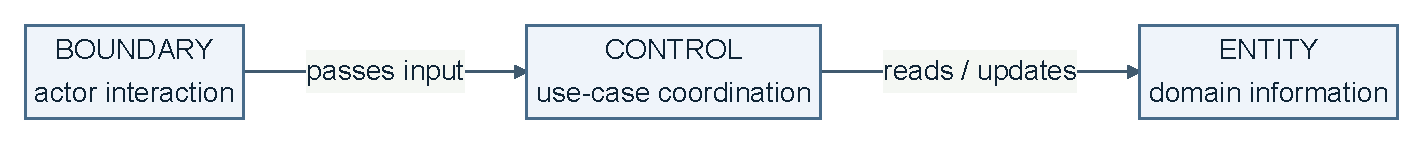
\includegraphics[width=419.06pt]{images/fig-005.pdf}
\captionof{figure}{assign each class a responsibility}\end{minipage}\par\smallskip



The boundary/control/entity arrows show a common collaboration, not every allowed relationship; derive responsibilities from the case.


\Needspace{4\baselineskip}
\subsection*{4.1 Elicitation vs analysis (L5 distinction)}
\sectionlabel{h-41-elicitation-vs-analysis-l5-distinction}


{\fontsize{9}{11}\selectfont
\begin{longtable}{L{\dimexpr 0.19613\linewidth-4.71pt\relax}L{\dimexpr 0.35448\linewidth-8.51pt\relax}L{\dimexpr 0.44939\linewidth-10.79pt\relax}}
\toprule
\rowcolor{ice}\textbf{} & \textbf{\textbf{Requirements elicitation}} & \textbf{\textbf{Requirements analysis}} \\
\midrule\endfirsthead
\toprule\rowcolor{ice}\textbf{} & \textbf{\textbf{Requirements elicitation}} & \textbf{\textbf{Requirements analysis}} \\
\midrule\endhead
\multicolumn{3}{r}{\scriptsize Continued on next page}\\\endfoot
\bottomrule\endlastfoot
Purpose & Find out \textbf{what customers want} & Produce a system model that is \textbf{correct, complete, consistent, unambiguous} based on the use cases \\
Output & Description of the system in terms of \textbf{actors and use cases} & \textbf{Conceptual model} (system structure) + \textbf{dynamic model} (system behaviour) \\
Perspective & Customer's & Software engineer's \\
Artefacts & SRS, use case diagram + descriptions, data dictionary, prototype & Class diagram (boundary/\allowbreak{}control/\allowbreak{}entity), sequence diagrams, state machines, activity diagrams \\
\end{longtable}
}

Formalising requirements with analysis models: \textbf{clarifies} structure and dynamics, \textbf{validates} requirements, \textbf{underpins} solution modelling.


\Needspace{4\baselineskip}
\subsection*{4.2 Conceptual model vocabulary}
\sectionlabel{h-42-conceptual-model-vocabulary}


{\fontsize{9}{11}\selectfont
\begin{longtable}{L{\dimexpr 0.21676\linewidth-5.20pt\relax}L{\dimexpr 0.37413\linewidth-8.98pt\relax}L{\dimexpr 0.40912\linewidth-9.82pt\relax}}
\toprule
\rowcolor{ice}\textbf{Element} & \textbf{Definition} & \textbf{Example} \\
\midrule\endfirsthead
\toprule\rowcolor{ice}\textbf{Element} & \textbf{Definition} & \textbf{Example} \\
\midrule\endhead
\multicolumn{3}{r}{\scriptsize Continued on next page}\\\endfoot
\bottomrule\endlastfoot
\textbf{Object} & Anything that has a \textbf{state} and exhibits \textbf{behaviour} & Bus, Dog, Company; \emph{LoginForm, UserVerifier, UserList} \\
\textbf{Operation} & Procedure through which objects communicate & Bus: Stop, Start; Company: Sell, Quote; UserVerifier: authenticate \\
\textbf{Attribute} & Variable holding state information & Bus: Seats, Colour; Company: Name, Employees \\
\end{longtable}
}

\begin{studycolumns}
\vspace{0pt}

Documented in a \textbf{class diagram}: Object \ensuremath{\rightarrow} Class; Roles of the object \ensuremath{\rightarrow} Attributes and methods of the class.


\needspace{152pt}
\subsection*{4.3 Class notation}
\sectionlabel{h-43-class-notation}

\par\smallskip\noindent\begin{minipage}{\linewidth}\centering
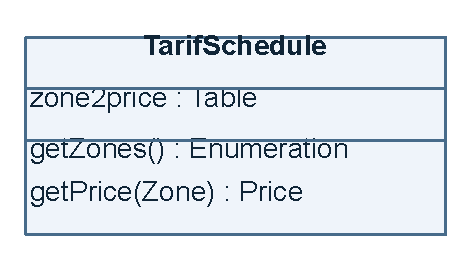
\includegraphics[width=138.46pt]{images/fig-006.pdf}
\captionof{figure}{4.3 Class notation}\end{minipage}\par\smallskip


\end{studycolumns}
\Needspace{110pt}
\subsection*{4.4 Relationships --- notation and reading}
\sectionlabel{h-44-relationships--notation-and-reading}

\needspace{4\baselineskip}
\subsubsection*{What the relationships look like}
\sectionlabel{h-what-the-relationships-look-like}
The following are concrete class-diagram sketches. Read the symbol \textbf{at the end of the line} carefully: that is where the relationship is attached.


\begin{center}
\begin{minipage}[t]{.235\linewidth}\centering\small\textbf{Association: structural link; navigation unspecified}\par\smallskip
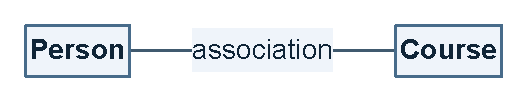
\includegraphics[width=.88\linewidth,height=75pt,keepaspectratio]{images/fig-007.pdf}\end{minipage}
\hfill
\begin{minipage}[t]{.235\linewidth}\centering\small\textbf{Navigability: reach the arrow-end class}\par\smallskip
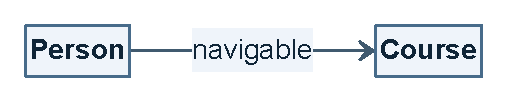
\includegraphics[width=.88\linewidth,height=75pt,keepaspectratio]{images/fig-008.pdf}\end{minipage}
\hfill
\begin{minipage}[t]{.235\linewidth}\centering\small\textbf{Non-navigable: Person cannot reach Course}\par\smallskip
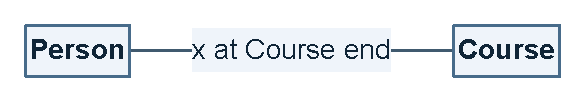
\includegraphics[width=.88\linewidth,height=75pt,keepaspectratio]{images/fig-009.pdf}\end{minipage}
\hfill
\begin{minipage}[t]{.235\linewidth}\centering\small\textbf{Generalization: triangle at parent; no multiplicity}\par\smallskip
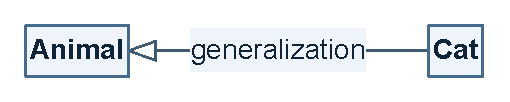
\includegraphics[width=.88\linewidth,height=75pt,keepaspectratio]{images/fig-010.pdf}\end{minipage}
\par\medskip
\begin{minipage}[t]{.235\linewidth}\centering\small\textbf{Abstract superclass: cannot instantiate}\par\smallskip
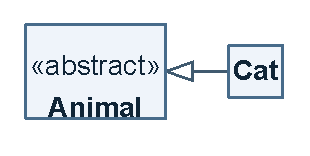
\includegraphics[width=.88\linewidth,height=75pt,keepaspectratio]{images/fig-011.pdf}\end{minipage}
\hfill
\begin{minipage}[t]{.235\linewidth}\centering\small\textbf{Realization: implements an interface}\par\smallskip
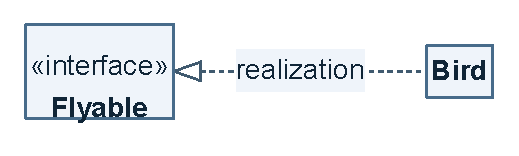
\includegraphics[width=.88\linewidth,height=75pt,keepaspectratio]{images/fig-012.pdf}\end{minipage}
\hfill
\begin{minipage}[t]{.235\linewidth}\centering\small\textbf{Aggregation: parts can outlive the whole}\par\smallskip
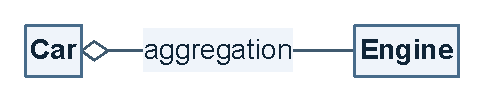
\includegraphics[width=.88\linewidth,height=75pt,keepaspectratio]{images/fig-013.pdf}\end{minipage}
\hfill
\begin{minipage}[t]{.235\linewidth}\centering\small\textbf{Composition: exclusive ownership and lifecycle}\par\smallskip

\includegraphics[width=.88\linewidth,height=75pt,keepaspectratio]{images/fig-014.pdf}\end{minipage}
\par\medskip
\begin{minipage}[t]{.235\linewidth}\centering\small\textbf{Dependency: temporary use}\par\smallskip
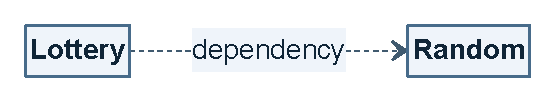
\includegraphics[width=.88\linewidth,height=75pt,keepaspectratio]{images/fig-015.pdf}\end{minipage}
\hfill
\begin{minipage}[t]{.235\linewidth}\centering\small\textbf{Multiplicity: near-end class is counted}\par\smallskip
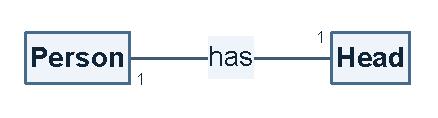
\includegraphics[width=.88\linewidth,height=75pt,keepaspectratio]{images/fig-016.pdf}\end{minipage}
\par\medskip
\par\smallskip\small Mermaid cannot draw UML's non-navigable x; place it at the Course end in an examination drawing.\par
\captionof{figure}{Relationship notation atlas: read the symbol at each end.}
\end{center}
\begin{studycolumns}
\textbf{Multiplicity cheatsheet}


\begin{referenceentries}
\textit{\textbf{Notation} / \textbf{Meaning}}\par\smallskip
\noindent \textbf{\code{1}}: Exactly one\par
\noindent \textbf{\code{0.\allowbreak{}.\allowbreak{}1}}: Zero or one (optional)\par
\noindent \textbf{\code{*} or \code{0.\allowbreak{}.\allowbreak{}*}}: Zero or more\par
\noindent \textbf{\code{1.\allowbreak{}.\allowbreak{}*}}: One or more\par
\noindent \textbf{\code{3}}: Exactly three\par
\noindent \textbf{\code{1.\allowbreak{}.\allowbreak{}6}}: Between one and six\par
\end{referenceentries}
\textbf{How to read a multiplicity correctly:} the number is written \textbf{at the end near the class it counts}. \code{Person "1" -\allowbreak{}-\allowbreak{} "1" Head} means one Head per Person and one Person per Head. \code{Polygon "1" -\allowbreak{}-\allowbreak{} "*" Point} means zero or more Points per Polygon and one Polygon per Point.

\textbf{Notation:} abstract class names are italicised or marked \code{\{abstract\}}; interface realisation uses a dashed line and hollow triangle.

\par\smallskip{\color{amber}\bfseries Traps and things to check}\par
Choose one relationship type per line. Generalization has a hollow triangle at the parent, no multiplicities or role names. Association multiplicities belong at both counted ends. A plain line leaves navigability unspecified; an x prohibits reaching its target end. Composition adds exclusive composite ownership and lifecycle responsibility; a part may be detached before deletion. Use hollow-triangle generalization despite L5's inconsistent filled-arrow example.
\par\smallskip
\end{studycolumns}

\Needspace{4\baselineskip}
\subsection*{4.5 Stereotypes: entity /\allowbreak{} boundary /\allowbreak{} control}
\sectionlabel{h-45-stereotypes-entity--boundary--control}


{\fontsize{9}{11}\selectfont
\begin{longtable}{L{\dimexpr 0.22883\linewidth-5.49pt\relax}L{\dimexpr 0.36549\linewidth-8.77pt\relax}L{\dimexpr 0.40568\linewidth-9.74pt\relax}}
\toprule
\rowcolor{ice}\textbf{Stereotype} & \textbf{Role} & \textbf{Typical examples} \\
\midrule\endfirsthead
\toprule\rowcolor{ice}\textbf{Stereotype} & \textbf{Role} & \textbf{Typical examples} \\
\midrule\endhead
\multicolumn{3}{r}{\scriptsize Continued on next page}\\\endfoot
\bottomrule\endlastfoot
\textbf{\guillemotleft{}entity\guillemotright{}} & Information tracked by the system & \code{Account}, \code{Silo}, \code{Shipment} \\
\textbf{\guillemotleft{}boundary\guillemotright{}} & Interaction between an actor and the system & \code{Login\allowbreak{}Form}, \code{Entry\allowbreak{}Gate}, \code{Fingerprint\allowbreak{}Reader} \\
\textbf{\guillemotleft{}control\guillemotright{}} & Logic that realises a use case (coordination) & \code{Facility\allowbreak{}Access\allowbreak{}System}, \code{Sheet\allowbreak{}Manager}, \code{Registration\allowbreak{}Controller} \\
\end{longtable}
}

\begin{studycolumns}
\vspace{0pt}

Worked example --- \textbf{EnterSecureFacility}:


\begin{quote}\small\color{navy}
\begin{enumerate}
\item User presses finger on FingerprintReader. 2. FingerprintReader scans and sends image to FacilityAccessSystem. 3. FacilityAccessSystem validates fingerprint and unlocks EntryGate.
\item EntryGate signals the system it has opened. 5. FacilityAccessSystem locks EntryGate, logs the entry event and increments occupant count.
\end{enumerate}
\end{quote}
Classes: \code{Employee} (\guillemotleft{}entity\guillemotright{}), \code{Fingerprint} (\guillemotleft{}entity\guillemotright{}), \code{Fingerprint\allowbreak{}Reader} (\guillemotleft{}boundary\guillemotright{}), \code{Entry\allowbreak{}Gate} (\guillemotleft{}boundary\guillemotright{}), \code{Facility\allowbreak{}Access\allowbreak{}System} (\guillemotleft{}control\guillemotright{}). Relations with stereotypes: \code{<<read>\allowbreak{}>\allowbreak{}}, \code{<<call>\allowbreak{}>\allowbreak{}}, \code{<<signal>\allowbreak{}>\allowbreak{}} (usage dependencies between them).


\needspace{4\baselineskip}
\subsection*{4.6 Four-step analysis procedure}
\sectionlabel{h-46-four-step-analysis-procedure}
\begin{enumerate}
\item Identify the \textbf{classes}.
\item Find the \textbf{attributes} for each class.
\item Find the \textbf{methods/\allowbreak{}operations} for each class.
\item Find the \textbf{associations} between classes.
\end{enumerate}
How to find classes:

\begin{enumerate}
\item \textbf{Recurring nouns/\allowbreak{}concepts} in the use cases.
\item \textbf{Real-world entities} the system must track.
\item \textbf{Application/\allowbreak{}problem-domain terms} in the data dictionary. Then \textbf{review definitions and attributes with stakeholders}.
\end{enumerate}

\begin{quote}\small\color{navy}
\textbf{Trap:} do \textbf{not} promote every noun to a class. If a noun has no attributes, no identity and no behaviour of its own (e.g. "amount", "date", "grade"), it is an \textbf{attribute}, not a class. Conversely "grade" in GES has an enumerated domain and constrains storage rules \ensuremath{\rightarrow} it can justify a class/\allowbreak{}type in the design model.

\end{quote}
\end{studycolumns}
